\FloatBarrier
\subsection{LetterLizardJS: JavaScript Letter Lizard Implementation}

% Introduce Language
% JAVASCRIPT
% - "language of the Web", implemented in Web browsers to allow client 
%   side scripts to interact with the user, control browser, preform 
%   asynchrous communication with server, alter docmuent that is displayed
% - also server-side programming, desktop and mobile applications
% - dynamic, prototype based
% - first class functions
% - syntax influenced by C, Java, but very different
% - key design principles takes from Self, Scheme
% - multi-paradigm: oop, imperative, functional
% - first introduced by Netscape, formalized as ECMAScript 

JavaScript is the ``language of the Web'' and has become an indispensable 
tool for Web developers. Client-side JavaScript scripts executed in Web
browsers are able to bring life to Web pages by interacting with the user,
controlling the behaviour of the browser, performing asynchronous communication
with Web servers and altering the document that is displayed. Although originally
introduced by Netscape for client-side scripting in 1995, it is increasingly
more common for JavaScript to be used in other contexts as well. For example,
a recent trend has been to implement server-side applications in JavaScript as
has been demonstrated by the explosion in popularity of Node.js~\cite{nodejs} and other
server-side JavaScript frameworks. Not long after Netscape started shipping 
JavaScript in its Navigator browser, it submitted the language to Ecma International
and it is now standardized as ECMA-262 and known as ECMAScript.
There are several well-known implementations of the language that conform to the standard.

% - supports structured programming like C
% - exeption: function scoping instead of block scoping
% - many think that this was not a good idea (cite Definitive guide?)
% - automatic semicolon insertion (also not a good idea) (cite def guide?)
% - dynamic typing: types associated vith values, not variables
% - object based: objections are associative arrays with String or int
%   property names (special langauge support for arrays)
% - aside from a few primitive types, everything is an object, including
%   funcions (which means that funcitons are first-class enitiies - they
%   can be assigned to variables and even returned from other functions
% - event driven; 1st class funcs used a lot in event-driven browser/
%   run-time environment
% - closures (give an example or refer to later section)
% - objects augmented with prototypes; can be used to simulate "classical"
%   oop features
% - no distinction between func and method: caling convention


JavaScript is a dynamic, prototype-based object oriented language with first-class
functions. Much of its syntax has been influenced by C, C++ and Java, but
the languages are actually very different. JavaScript borrows key design principles
from Self and Scheme. JavaScript supports several different programming
paradigms including object-oriented, imperative and functional. JavaScript supports
structured programming similar to C with many of the same flow-control statements
such as \texttt{if}, \texttt{for}, \texttt{while}, etc. One notable difference,
however, is the lack of block scoping for variables. Instead, JavaScript 
uses function scoping
for variables, which means that all variable declared in a function are
visible throughout the entire body of the function. This means that 
variables are even visible before they are declared. This feature 
is known as ``hoisting:'' JavaScript code behaves as if all variable 
declarations in a function are hoisted to the top of the function. This ``feature''
can easily cause bugs that are hard to find when local variables shadow variables in
an outer scope, and for this reason it is considered a negative aspect of the 
language~\cite{goodparts}. JavaScript also contains a mechanism that tries to
correct faulty programs by automatically inserting semicolons to complete statements, but quite
often this masks more serious errors~\cite{goodparts} or results in unexpected behaviour.
We explore these issues further in sections~\ref{varscope} and~\ref{exprandstmt} respectively.

JavaScript has a dynamic type system in which types are associated with values,
not variables. A few primitive types are provided by the language, such
as Number, String, Boolean, null and undefined. Aside from the primitive types,
everything else is an Object. Objects are composite types
that are comprised of properties: name-value pairs where the name is a String
(or an integer for arrays, we will see more about this in section~\ref{objects})
and the value is one of the primitive types or another object. Even functions
are objects (with associated behaviour), which means that functions are first-class
entities that may be assigned to variables and returned from other functions.

Each JavaScript function also contain a reference to the scope chain that was
in effect when the function was defined, which is used to resolve variable
names to values when the function is executed. A function, together with a
reference to its scope chain is know as a \emph{closure} (we will cover closures
in section~\ref{closures}). 
JavaScript usually runs in event-driven environments, such as the client-side
environment of a Web browser, that make heavy use of closures and first-class 
functions for callbacks.

JavaScript supports object-oriented programming, but not in the classical
sense. Rather than providing class-based inheritance, JavaScript provides
\emph{prototype-based inheritance}. Every object has as second object (or,
in some rare cases, \emph{null}) associated with it. This second object is
know as its \emph{prototype}, and the first object inherits properties from
its prototype. Many programmers who are new to JavaScript who come from a
C, C++, or Java background find JavaScript's prototype-based inheritance
confusing at first; however, it is really quite simple and works nicely
JavaScript's dynamic nature. Most classical object-oriented features can be
easily simulated in JavaScript. We discuss object-oriented programming
in section~\ref{oop}.

\begin{figure}
    \centering
	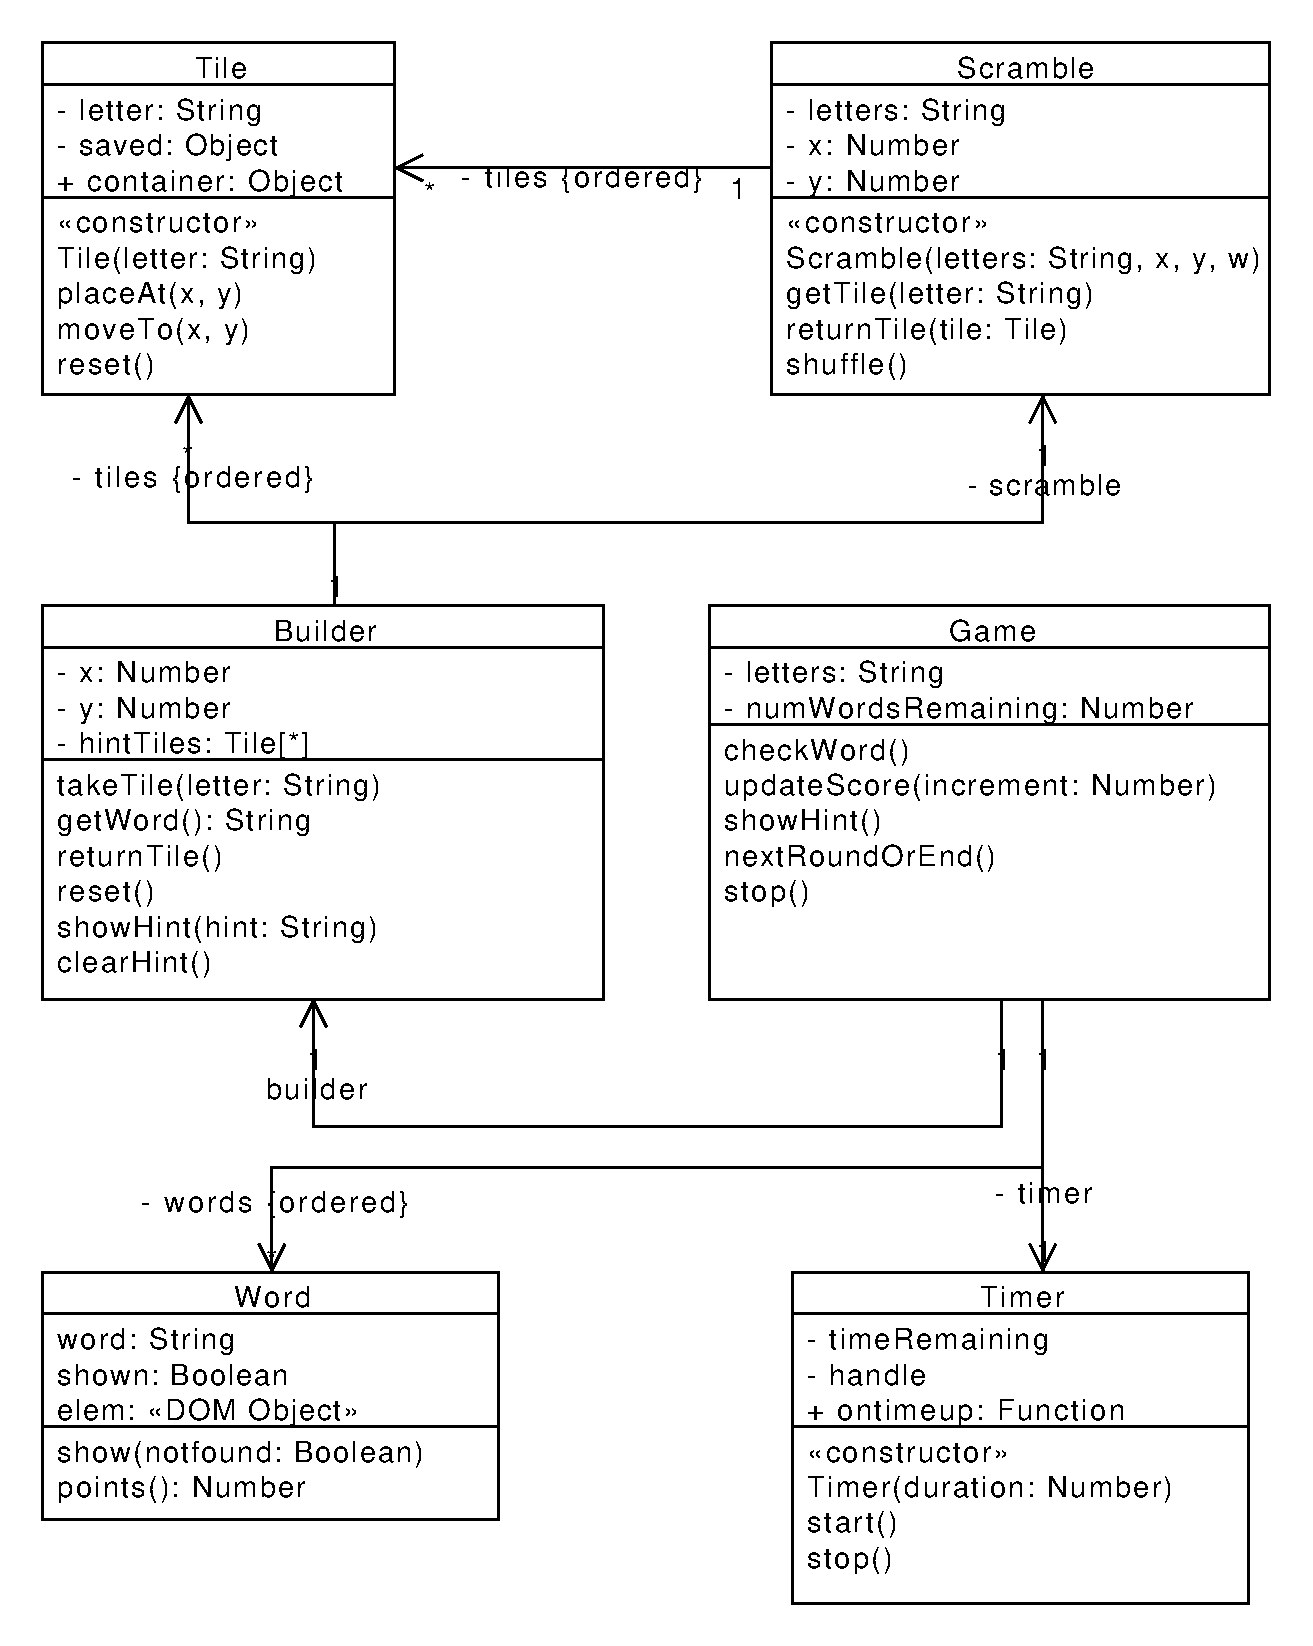
\includegraphics[scale=0.6]{../diagrams/LetterLizardJS-ClassDiagram.pdf}
	\caption{A class diagram showing the classes that make up the JavaScript Letter
	Lizard implementation. The event-driven, callback-based client-side scripting
	environment naturally led to a modularized, class-based design for the game.}
\end{figure}


% talk about how this version is implemented (eg classes, etc)
% show screenshots
% talk about implementation: language features that were useful,
% class diagrams, sequence diagrams, snippets of code, etc